The top squarks are said to stabilize the Higgs mass and since the eigenstates of the stops mix strongly, they are significantly lighter than other squarks ($m_{\Tilde{t}_1} \ll m_{\text{squarks}}$) \cite{arbey2012higgs}. Considering stops as the next-lightest SUSY particle allows the LSP (potentially a neutralino) to be produced, making stops an ideal candidate for the next detection in collider experiments.
%-------------------------------------------------------------------------%
\section{Masses of stop particles}
Mass eigenstates of the squarks and sleptons of the MSSM can be obtained by diagonalizing three $6\times6$ (from the up- and down-type squarks and charged sleptons) and one $3\times3$ matrices (from sneutrinos) of which most are negligible due to their small mixing angles \cite{martin1997supersymmetry}. For the stops, in particular, the mass eigenstates are given by the matrices

\begin{align}
    \begin{pmatrix} \Tilde{t}_1 \\ \Tilde{t}_2 \end{pmatrix} = 
    \begin{pmatrix} \cos\theta_\Tilde{t} & -\sin\theta^*_\Tilde{t} \\ \sin\theta_\Tilde{t} & \cos\theta^*__\Tilde{t} \end{pmatrix}
    \begin{pmatrix} \Tilde{t}_L \\ \Tilde{t}_R \end{pmatrix}
    \label{eq:stopMass}
\end{align}
where $ \theta_\Tilde{t} $ is the stop mixing angle in the range $ 0 \leq {\theta_\Tilde{t}} \leq \pi $ satisfying $ |\cos\theta_{\Tilde{t}}|^2 + |\sin\theta_{\Tilde{t}}|^2 = 1 $. \\

The mass splitting of the two stops $ \tilde{t}_1 $ and $ \tilde{t}_2 $ arise from the squared-mass matrix for stops shown in Equation (\ref{eq:stopMatrix}), where the off-diagonal elements involves a large top-quark Yukawa coupling ($y_t$ term) that induces such a phenomena \cite{kraml2016scalar}. Diagonalizing Equation (\ref{eq:stopMatrix}) gives the $\Tilde{t}_L$ and $\Tilde{t}_R$ components on the right-hand side of Equation (\ref{eq:stopMass}). \\

%The Lagrangian for the gauge-eigenstate is given by

%\begin{align}
 %   \Lagr_\text{stop masses} = 
  %  - \begin{pmatrix} \Tilde{t^*}_L & \Tilde{t^*}_R \end{pmatrix} \mathbf{m^2_\Tilde{t}} \begin{pmatrix} \Tilde{t}_L \\ \Tilde{t}_R \end{pmatrix}
   % \label{eq:stopLag}
%\end{align}

%where
\begin{align}
    \mathbf{m^2_\Tilde{t}} =
    \begin{pmatrix}
    m^2_{Q_3} + m^2_t + \Delta_{\Tilde{u}_L} & v(a^*_t\sin\beta - \mu y_t \cos\beta) \\
    v(a_t\sin\beta - \mu^2 y_t \cos\beta) & m^2_{\Bar{u}_3} + m^2_t + \Delta_{\Tilde{u}_R}
    \end{pmatrix}
    \label{eq:stopMatrix}
\end{align}

Here, the terms not yet menioned are \cite{martin1997supersymmetry, arbey2012higgs}:
\begin{itemize}
  \item $m^2_{t}$ = squared mass of the top quark
  \item $m^2_{Q_3}$ = squared mass of the third-family squark
  \item $ m^2_{\Bar{u}_3}$ = squared mass of the third-family sleptons
  \item $\Delta_{\Tilde{u}_L/R}$ = contribution from the sleptons to the mass
  \item $a_t$ = soft scalar coupling term
  \item $v$ = vacuum expectation value (VEV) of the Higgs
  \item $\mu$ = Higgs-Higgsino mass parameter
  \item $\beta$ = VEV coupling angle. By convention, $0 < \beta < \pi/2$
\end{itemize}

%The mass eigenstates are then obtained by diagonalizing (\ref{eq:stopMatrix}) using a unitary matrix, giving

Due to many reasons out of the scope of this review, various models predict that $\Tilde{t}_1$ is the lightest of all squarks, predominantly theorized to be $\Tilde{t}_R$ which is the right-handed stops \cite{martin1997supersymmetry}. Although there has been no success in the direct detection, therefore, a properly theorized mass, experimental efforts have been made to set constraints for the stop mass \cite{kraml2016scalar, aad2014search, abdughani2018probing, sirunyan2018search, yoshihara2017search}.
%-------------------------------------------------------------------------%
\section{Possible decay channels of the top squarks} \label{sec:stopDecay}

Just like the SM particles and their decay dictated by known symmetries and conservation laws, the decay of stops is dictated by the parameters and kinematics suggested by MSSM. The mass of stops would significantly affect the decay modes. \\

A heavy enough stop at the order of the sum of the top quark mass and neutralino mass ($m_t+m_{\Tilde{\chi}_1^0}$)(or charginos) would undergo a two-body decay into top quarks with neutralinos: $\Tilde{t}_1\rightarrow t\Tilde{\chi}_1^0$ (or bottom quarks with charginos: $\Tilde{t}_1\rightarrow b\Tilde{\chi}_1^+$) \cite{boehm2000decays}. A lighter stop that is above the sum of the bottom quark mass, W-boson mass and neutralino mass ($m_b + m_W + m_{\Tilde{\chi}_1^0}$) would imply a three-body decay $\Tilde{t}_1\rightarrow b W \Tilde{\chi}_1^0$ \cite{aad2014search}. Four-body decays into a combination of bottom quarks, neutralinos and SM fermions, may also be possible: $\Tilde{t}_1\rightarrow b\Tilde{\chi}_1^0 f \Bar{f}'$ \cite{boehm2000decays}. However, the four-body decay is only relevant when the two- and three-body decays are kinematically forbidden i.e. on-shell decays aren't allowed. This would also allow a flavor-suppressed decay to a charm quark: $\Tilde{t}_1\rightarrow c\Tilde{\chi}_1^0$ \cite{aad2014search}, where both this decay and the four-body decay can be very slow such that $\Tilde{t}_1$ is quasi-stable \cite{martin1997supersymmetry}. \\

An important assumption made in these decays is that $m_{\Tilde{t}_1} > m_{\Tilde{\chi}_1^0} $ so that the neutralinos remain the lightest (LSP). Additional decays become apparent when sparticles other than $\Tilde{\chi}_1^0 $ are lighter than the stop, such as the charginos $\Tilde{\chi}_1^{\pm}$.
A diagram from \cite{aad2014search} is shown in Figure \ref{fig:decayMode}, that represent the above statements under the assumption that $\Tilde{t}_1 $ and $ \Tilde{\chi}_1^0 $ are both the lightest sparticles, which could very well not be true since there is no experimental evidence to disprove nor prove as such. 




\begin{figure}[htbp]
    \centering
    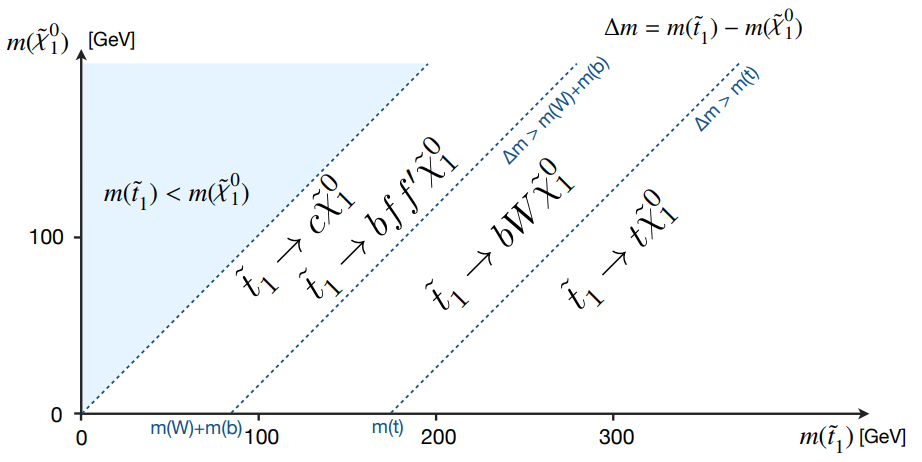
\includegraphics[width=15cm, height= 7.5cm]{decaymodes.png}
    \caption{Possible decay modes for stops within the mass-parameter-space of $\Tilde{t}_1 $ and $ \Tilde{\chi}_1^0 $ \cite{aad2014search}.}
    \label{fig:decayMode}
\end{figure}

\begin{figure}[htbp]
    \centering
    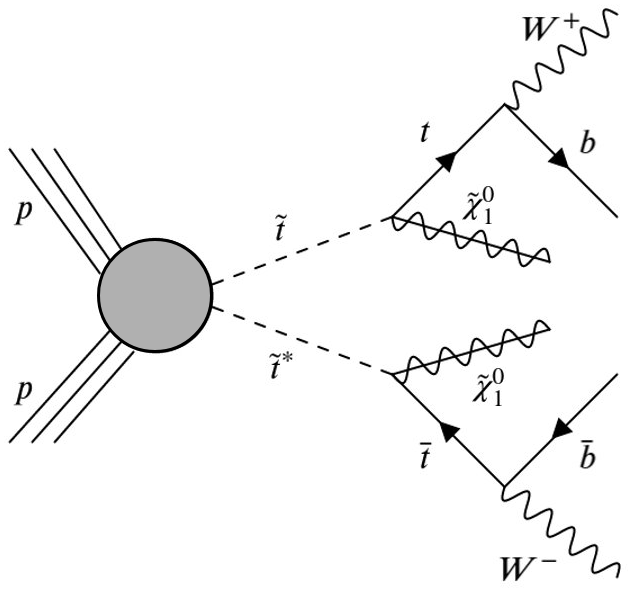
\includegraphics[width=9cm, height= 7.5cm]{stops_true.png}
    \caption{Decay chain of the signal of interest $\Tilde{t}_1 \rightarrow t\Tilde{\chi}_1^0 $.}
    \label{fig:decayInterest}
\end{figure}